\section{Introduction}

Deep neural networks received much success in many domains in the past years, and deeper architectures are adopted because of the complex application scenarios. However, since the memory and computational cost increase with the depth of network linearly, data parallelism across multiple devices is deployed to speed up the training process, whereas it is passively switch to data-model coupled parallelism because of the Batch Normalization (BN) layer\cite{ioffe2015batch}. The BN layer is generally introduced into the deep neural networks because of its significant margin no matter for rate of convergence or maximum of training accuracy. However, the mean and variance computed in this layer only stands for the sub mini-batch of one specific device, resulting in the separately model training of each device. The data-model coupled parallelism leads to that the model is trained with mini-batch size, rather than original batch size, and the training accuracy is influenced correspondingly.

\begin{figure}[b]
    \begin{center}
    \fbox{\includegraphics[width=0.8\linewidth]{figure/noreduce.png}}
    \caption{Data-model parallelism resulting from batch normalization layer}%
    \label{fig:localBN}
    \end{center}
    \end{figure}

To obtain global mean and variance, communication across all devices is required in each BN layer, which reduces the training speed greatly. As is well-known that the training accuracy increases with batch size generally and there exists a threshold after which the quality of model will be deteriorated\cite{keskar2016large}. Therefore, for large batch size cases such as imagenet\cite{krizhevsky2012imagenet}, the training accuracy loss resulting from local mean and variance is negligible compared to the communication cost. However, for memory-bounding cases such as semantic segmentation training on cityscapes dataset in self-driving field, the mini-batch size is only 3 at most with ResNet-50 in single GPU, and the training result is greatly limited under the original BN algorithm.


% The data-model coupled parallelism leads to that the model is trained with mini-batch size, rather than original batch size, and the training accuracy is influenced correspondingly. As is well-known that the training accuracy increases with batch size generally and there exists a threshold after which the quality of model will be deteriorated\cite{keskar2016large}. For memory-bounding cases such as semantic segmentation training on cityscapes dataset, the mini-batch size is only 3 at most with ResNet-50 in single GPU, and the training result is greatly limited under the original BN algorithm. Therefore, communication across multiple devices is essential to guarantee the  thoroughly data parallelism. While for large batch size cases such as imagenet\cite{krizhevsky2012imageneti}, the training accuracy loss is negligible compared to the communication cost.

% the batch size is limited by the GPU memory. As is well-known that the training accuracy increases with batch size generally and there exists a threshold after which the quality of model will be deteriorated\cite{keskar2016large}. Data parallelism across multiple devices enables us to break through the memory limitation.

% As is well-known that the training accuracy increases with batch size generally and there exists a threshold after which the quality of model will be deteriorated\cite{keskar2016large}, hence the memory becomes the bottleneck of deep learning under small-batch regime. In our semantic segmentation training on cityscapes dataset, the batch size is only 3 at most with ResNet-50 in single GPU, and the training result is greatly limited. 

% Data parallelism with multiple devices enables us to break through the memory limitation, whereas it is passively switch to data-model coupled parallelism because of the Batch Normalization (BN) layer\cite{ioffe2015batch} as is shown in figure\ref{fig:localBN}. The BN layer is generally introduced into the deep neural networks because of its significant margin no matter for rate of convergence or maximum of training accuracy. However, the mean and variance computed in this layer only stands for the sub mini-batch of one specific device, resulting in the separately model training of each device. Therefore, the training accuracy cannot reach the theoretical value under the original BN algorithm.



The aim of the study is achieving the balance between accuracy and efficiency. We need to reduce the cost between GPU's communication, so we propose and implement an adaptive global batch normalization (AGBN) algorithm across multi-GPUs. In the AGBN algorithm, variables such as mean and variances are computed based on the data across the whole devices to realize thoroughly data parallelism. Here the "adaptive" has two meanings: the AGBN algorithm degrades into the original BN algorithm (1) under large-batch regime; (2) until the training accuracy converges. The communication across devices is avoided as much as possible to improve the training efficiency.

% The aim of the study is to propose and implement a new strategy of performing batch normalization globally across multi-GPUs, furthermore to realize thoroughly data parallelism and then increase the training accuracy to theoretical value.



\section{Related work}

The distribution of each layer's inputs changing during training makes it complicated to train deep neural network. We used to be careful about parameter initialization and lowering learning rate.Batch Normalization\cite{ioffe2015batch} was put forward to solve this "interval covariate shift" phenomenon. The idea is normalize the inputs to layers within the network and apply a transformation that makes the mean close to 0 and standard deviation close to 1. Batch Normalization brings those benefits:network training faster, higher learning rate, easier weights initialization, provide some regularisation, etc.


Parameter server\cite{muli-ps} is a framework for distributed machine learning problems, and has been deployed in MXNET, an open-source, flexible and efficient library for Deep Learning\cite{chen2015mxnet}. Parameter server has a server group and several worker groups. A server node maintains a part of the globally sharesd parameters and a worker stores a piece of training data. Workers only communicate with server nodes not among themselves for updating or retrieving the shared parameters.


% \begin{figure}[h]
%     \begin{center}
%     \fbox{\includegraphics[width=0.8\linewidth]{figure/nccl_ring.png}}
%     \caption{Memonger optimized gradient graph generation exmaple }%
%     \label{fig:nccl-ring}
%     \end{center}
%     \end{figure}

\section{Methods}


This study is based on MXNET, and BN layer is treated as an operator here. The original BN algorithm consists of only one section:normalization. In our Global BN algorithm, we add two sections, pre-pocessing and reduce, and adjust normalization section accordingly to improve performance of BN algorithm.

\begin{figure}[h]
    \begin{center}
    \fbox{\includegraphics[width=0.8\linewidth]{figure/reduce.png}}
    \caption{Schematic of the process of global BN operator }%
    \label{fig:Memonger}
    \end{center}
\end{figure}

\subsection{Forward modification}

We first take a look at new forward prapagation in Global BN algorithm. In the pre-pocessing section, we compute the local mean and square of mean, here "local" means the output is computed from the data on the $i$th GPU, $m_i$ indicates the mini-batch size of the $i$th GPU. 
\begin{algorithm}[h]
    \caption{Forward Pre-processing}
    \label{alg:forward-pre}
    \begin{algorithmic}[1]
        \State For the $i$th GPU
        \State Input: $x_{i,j}$
        \State Output: $u_{i}$,$v_{i}$
        \State Get \textbf{local} mean and square of mean
        \begin{equation}
            {u_i} = \frac{1}{{{m_i}}}\sum\limits_{j = 1}^{{m_i}} {{x_{i,j}}} 
        \end{equation}
        \begin{equation}
            {v_i} = \frac{1}{{{m_i}}}\sum\limits_{j = 1}^{{m_i}} {x_{i,j}^2} 
        \end{equation}
    \end{algorithmic}
\end{algorithm}

%The last section is similar to the original BN algorithm except the operation of getting global variance and the output is identical to the original BN algorithm ignoring the reduce section as is shown in equation \ref{equ:normalization}.

In this section we compute the global mean and square of mean, and "global" means the output is based on the data of whole devices. $n$ indicates the count of devices.

\begin{algorithm}[h]
\caption{Forward Reduce} %算法的名字
\label{alg:forward-reduce}

\begin{algorithmic}[1]
\State Input: $u_{i}$,$v_{i}$
\State Output: $u$,$v$
\State Get \textbf{global} mean and square of mean
\begin{equation}
    {u = \frac{{\sum\nolimits_{i = 1}^n {{u_i}{m_i}} }}{{\sum\nolimits_{i = 1}^n {{m_i}} }}}
\end{equation}
\begin{equation}
    {v = \frac{{\sum\nolimits_{i = 1}^n {{v_i}{m_i}} }}{{\sum\nolimits_{i = 1}^n {{m_i}} }}}
\end{equation}
\end{algorithmic}
\end{algorithm}

The last part is batch normalization, which is similar to the original BN algorithm except the operation of getting global variance and the output is identical to the original BN algorithm ignoring the reduce section.

\begin{algorithm}[h]
\caption{Batch normalization} %算法的名字
\label{alg:forward-norm}
\begin{algorithmic}[1]
\State For the $i $th GPU
\State Parameter: $\gamma$,$\beta$
\State Input: $u$,$v$,$x_{i,j}$
\State Output: $y_{i,j}$
\State Get the output of BN layer:
\begin{equation}
    {\sigma ^2} = v - {u^2}
\end{equation}
\begin{equation}
    {\hat x_{i,j}} = \frac{{{x_{i,j}} - u}}{{\sqrt {{\sigma ^2} + \varepsilon } }}
\end{equation}
\begin{equation}
    {y_{i,j}} = \gamma {\hat x_{i,j}} + \beta 
\end{equation}
\end{algorithmic}
\end{algorithm}



% \begin{equation}
% \label{equ:reduce}
% \left\{ {\begin{array}{*{20}{c}}
% {u = \frac{{\sum\nolimits_{i = 1}^n {{u_i}{m_i}} }}{{\sum\nolimits_{i = 1}^n {{m_i}} }}}\\
% {v = \frac{{\sum\nolimits_{i = 1}^n {{v_i}{m_i}} }}{{\sum\nolimits_{i = 1}^n {{m_i}} }}}
% \end{array}} \right.
% \end{equation}
\subsection{Backward modification}

New backward propagation also consists of three parts. In pre-preprocessing part we need to calculate the mean of gradient $\psi_{i}$ and the mean of product of gradient and input data $\phi_{i}$ on $i$th device and store them.

\begin{algorithm}
    \caption{Backward pre-processing}
    \label{alg:backward-pre}
    \begin{algorithmic}[1]
        \State For the $i$th GPU
        \State Input: $\frac{\partial l}{\partial y_{i,j}}$,$x_{i,j}$$(j = 0,1,2\cdots n)$
        \State Output: $\psi_{i}$,$\phi_{i}$

        \begin{equation}
            {\psi_{i}} = {\frac{1}{m_{i}}} {\sum_{j=1}^{m_{i}} {\frac{\partial l}{\partial y_{i,j}}}}
        \end{equation}

        \begin{equation}
            {\phi_{i}} = {\frac{1}{m_{i}}} {\sum_{j=1}^{m_{i}} {\frac{\partial l}{\partial y_{i,j}}} \cdot {x_{i,j}}}
        \end{equation}
    \end{algorithmic}
\end{algorithm}


Then in reduce part, we will calculate the \textbf{global} mean of $\psi$ and $\phi$ across whole devices

\begin{algorithm}
    \caption{Backward reduce}
    \label{alg:backward-reduce}
    \begin{algorithmic}[1]
        \State Input: $\psi_{i}$,$\phi_{i}$,$m_{i}$$(i = 0,1,2\cdots n)$
        \State Output: $\psi$,$\phi$
        \begin{equation}
            {\psi} = {\frac{ \sum_{i=1}^{n} {\psi_{i}} {m_{i}} }{\sum_{i=1}^{n} {m_{i}}}}
        \end{equation}

        \begin{equation}
            {\phi} = {\frac{ \sum_{i=1}^{n} {\phi_{i}} {m_{i}} }{ \sum_{i=1}^{n} {m_{i}}}}
        \end{equation}
    \end{algorithmic}
\end{algorithm}


As for the batch normalization part is similar to the original BN algorithm except using $\psi$ and $\phi$ calculated in Backward reduce part.

\subsection{Data synchronization across GPUs}

Primary operation during the whole global batch normalization process is synchronize key data like mean and variance across all GPUs used in training.


% \section{model building}

% As we all know, we have to train a deep neural network for hundreds of epochs to make it converge, which means that communication overhead between GPUs in Global BN algorithm can not be ignored. In order to maximize the utilization of our multi-GPU machine, we want to build a training time prediction model to guide the training process. We divide the training process into two parts: computation cost and communication cost, and we will analyse them one by one.


% \subsection{Communication cost}

% Normally, communication between GPUs is done in the way that the data is sent from multiple GPUs to a single reducer GPU, which becomes the primary bottleneck in how fast the training can be done. It grows worse with data volume expanding. Baidu Research has brought up a new bandwidth-optimal allreduce algorithm named "Ring allreduce"\cite{baidu-allreduce} which drastically reduce the communication overhead. However, it is still constrained primarily by the slowest communication mechanism between devices like Infiniband, not by the number of GPUs now.

% Considering that we only use 8 GPUs at most for now, it is less likely to be dragged by the straggler. We apply Ring allreduce implemented in Nvidia Collective Communication Library\cite{jeaugey2017nccl} to accomplish data sychronization across all devices. NCCL implicitly indexes the GPUs into the optimal ring order under the hood. By taking topology of the interconnects between processors into account, it can achieve good performance for collectives communication.

% %add ring allreduce demo picture here

% \begin{algorithm}
%     \caption{Ring Allreduce}
%     \label{alg:ring-allreduce}
%     \begin{algorithmic}[1]
%         \State Set up communication ring
%         \State Divide array into N equal-size chunks
%         \State Scatter-reduce for N-1 iterations
%         \State Allgather for N-1 iterations
%     \end{algorithmic}
% \end{algorithm}

% Assume the total amount of data is M bytes, and it is evenly distributed among N GPUs. Each GPU does $2(N-1)$ iteraions and sends and receives M/N bytes data in each iteration, so each GPU sents and receives $2M*(N-1)/N$ bytes data during the whole allreduce process. If the bandwidth between GPUs is S byte/s, the expected time to finish allreduce is :
% \begin{equation}
%     CommTime = 2M*(N-1)/(N*S)
% \end{equation}


%  More importantly, because $(N-1)/N$ goes to $1$ with N growing larger, communication overhead for each GPU has a predictable and acceptable upper bound.

% \begin{table}[h]
    
%     \begin{tabular}{|c|c|c|c|}
%         \hline GPUs | data Size(MB) & 10 & 100 & 1000 \\
%         \hline  2 & 2.784 & 27.855 & 279.106 \\
%         \hline  3 &	3.693 &	36.805 &	370.472 \\
%         \hline 4 &	4.331 &	42.449 &	423.478 \\
%         \hline  5 &	4.638 &	46.119 &	458.021 \\
%         \hline  6 &	4.819 &	47.841 &	475.478 \\
%         \hline  7 &	5.001 & 48.934 &	489.464 \\
%         \hline  8 &	5.148 &	50.038 &	499.994 \\
%         \hline
%     \end{tabular}{}
%     \caption{Time(seconds) used to allreduce different sizes of data on multi-GPUs machine}
%     \label{tab:allreduce-overhead}
% \end{table}


% To validate our communication overhead prediction model, we did an data allreduce experiment on 8 GTX 1080Ti GPUs. As the table\ref{tab:allreduce-overhead} shows, the result of our experiment agrees well with our model. Communication time grows linearly with larger data size, and increases slower with more GPUs.



% \subsection{Computation cost}

% Deep neural network consists of many kinds of layers like convolutional/batch normalization/pooling/activation and so on. We would only focus on convolution layer here because other layers like fullyconnected and pooling layer often takes less than 10\% of the total time used in training a DNN .For any convolutional layer, its time complexity is :

% \begin{equation}
%     Flops \sim O(M^2 \cdot K^2 \cdot C_{in} \cdot C_{out})
% \end{equation}

% Here $M$ is the spatial size of the output feature map. $K$ is the length of the filter. $C_{in}$ is the number osf input channels of last layer. $C_{out}$ is the number of filters(also known as the output channels of this layer). Especially, M is determined by input matrix size $X$, length of the filter $K$, $Padding$ and $Stride$ (We assume the input and filters are square to simplify the expression):

% \begin{equation}
%     M = (X - K + 2 * Padding) / Stride + 1
% \end{equation}

% Because a convolutional neural network consists of many convolutional layers with different settings, we sum them up and get the total flops needed to:

% \begin{equation}
%     Flops \sim O(\sum_{l=1}^{D} M_{l}^{2} \cdot K_{l}^{2} \cdot C_{l-1} \cdot C_{l})
% \end{equation}

% Here $l$ is the index of a convolutional layer. $D$ is the number of convolutional layers\cite{kaiming-cnn-constrained-time}. In short, multiplication within layer and accumulation between layers. 

% \subsection{Other overhead}

% When we monitor the utilization of our GPUs using NVIDIA drivers, although it shows it is 100\% fully loaded, not all of its time is doing pure computation or data sychronization. There are 

% \subsection{Expected time prediction}




\section{Refinement}

As we all know, we have to train a deep neural network for hundreds of epochs to make it converge, which means that communication overhead between GPUs in Global BN algorithm can not be ignored. We evaluate the overhead by using 8 GTX 1080Ti GPU to  train image classification on Cifar10 dataset\cite{krizhevsky2014cifar} with ResNet-20. The table below shows how much time it takes to train one epoch on average.

% \begin{table}[!hbp]
    
%     \begin{tabular}{|c|c|c|c|}
%         \hline Batch size & Original/s & Global BN/s & Overhead ratio/\% \\
%         \hline    8 & 79.48  &  164.19  & 51.59 \\
%         \hline    16 & 60.72  &  91.32  & 33.51 \\
%         \hline    32 &  31.98   &  44.13  &  27.53 \\
%         \hline    64  &  16.53   &  23.48   & 29.60 \\
%         \hline    128  &  8.47  &  12.27  &  30.96 \\
%         \hline    256  &  4.21  &   7.32  &   42.49 \\
%         \hline
        
%     \end{tabular}
%     \caption{Time to train image classification on Cifar10 with ResNet-20 per epoch}
%     \label{tab:overhead}
% \end{table}

Obviously, the overhead from data sychronization across all devices occupies about $1/3$ of the total time of Global BN algorithm in most cases. Such high overhead from communication when training deep neural network exceeds what we can bear. We will propose several pratical strategies to reduce it to an affordable range later.

\begin{figure}[!hbp]
    \centering
    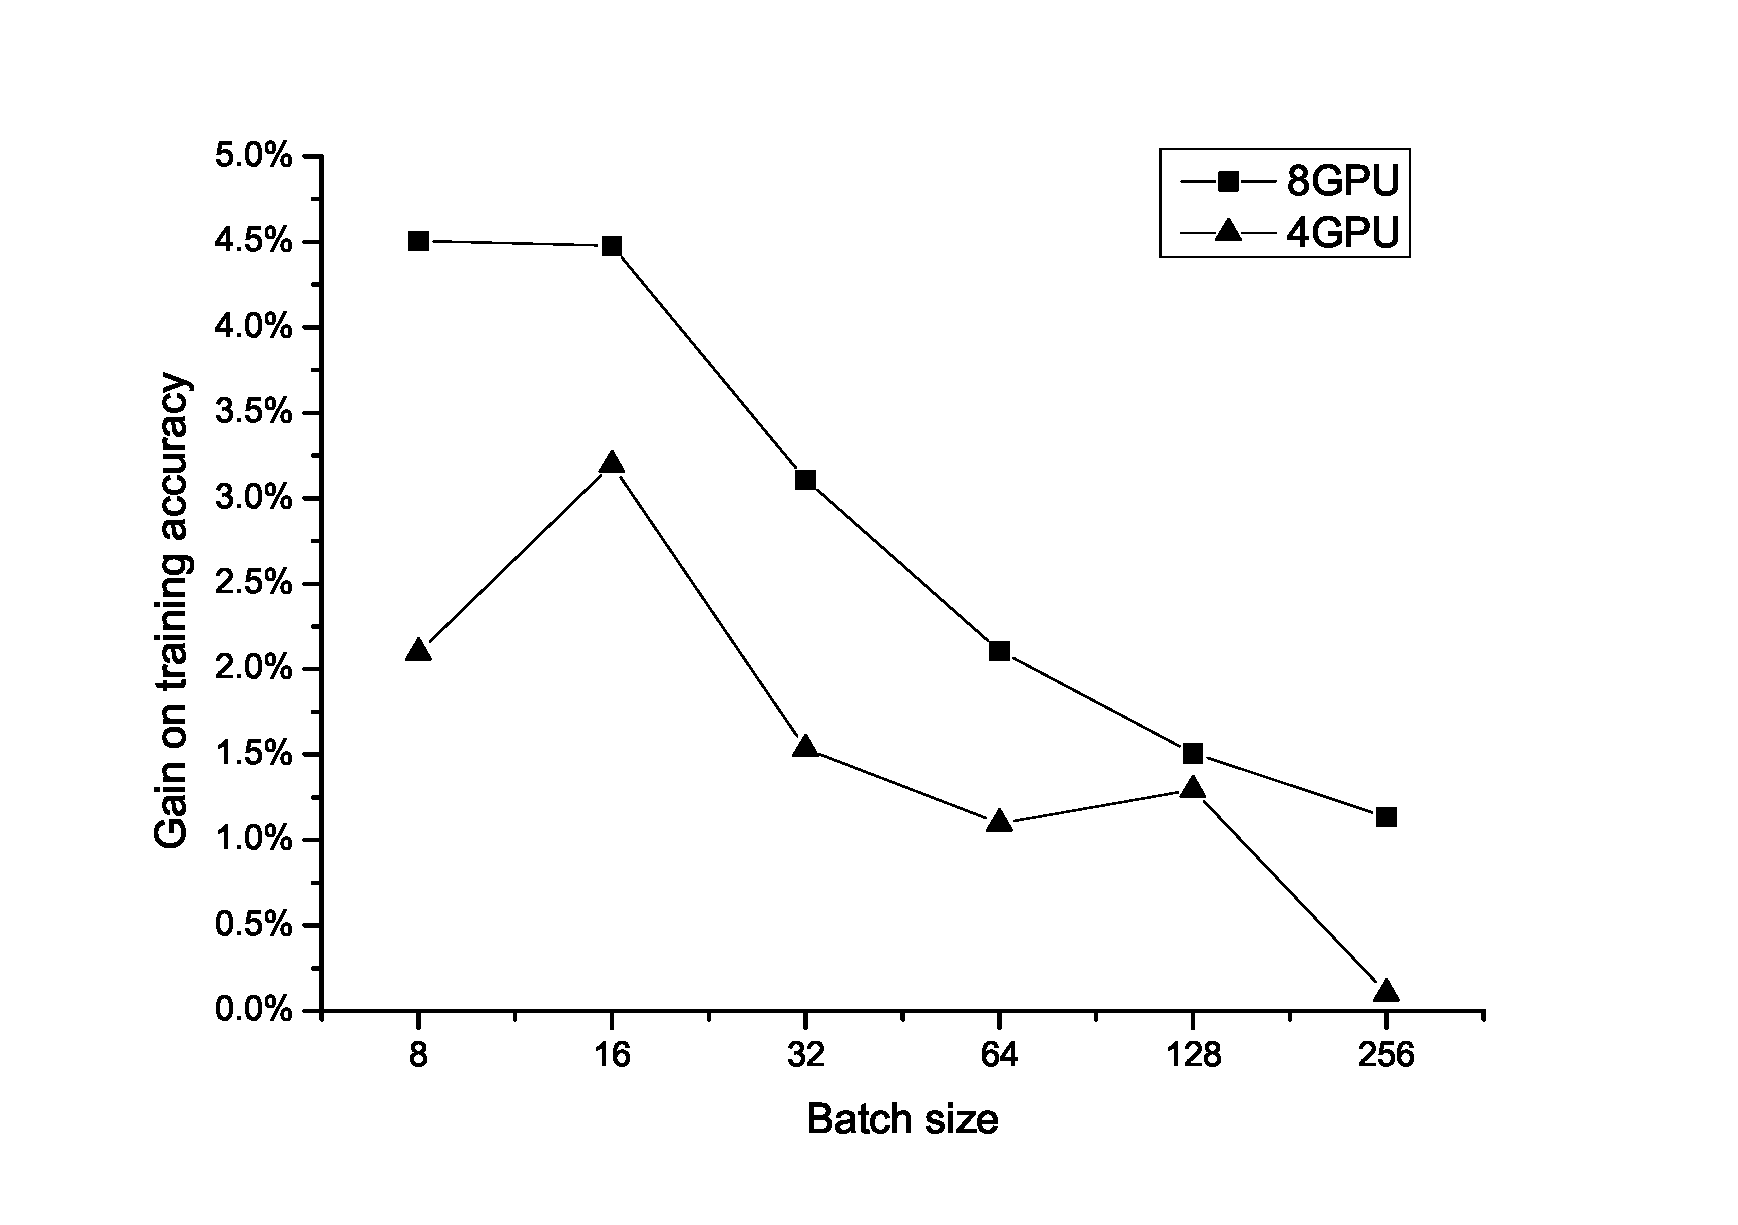
\includegraphics[width=0.8\linewidth]{figure/accVsBz.eps}
    \caption{Gain of Global BN algorithm on training accuracy under different batch sizes}
    \label{fig:accVsBz}
    \end{figure}

Also, We compare the gain on training accuracy of Global BN algorithm under different batch size as the figure \ref{fig:accVsBz} shows. The batch size is $BZ$ for the whole devices, so the mini-batch size in a single device $BZ_{mini}=BZ/n$, where $n$ indicates the count of devices. 
As we can see, for case $BZ=8$, the training accuracy raises about 2.1$\%$ and 4.4$\%$ for 4 devices and 8 devices, respectively. It is clear that the accuracy earning from data sychronization during batch normalization decreases monotonously as batch size grows no matter for 4 GPUs or 8 GPUs. Therefore, switch from GBN to original BN algorithm under 
large batch size case is appropriate to gain a trade-off between accuracy and efficiency.

% \subsection{Memory monger}

% Cifar10 dataset is a relatively small one. When deep neural network is applied in some real scenarios like Cityscapes,  the ResNet-50 mini-batch size on single GTX 1080Ti graphics card is 3 at most, which is far from enough. 

% Memonger\cite{tianqichen-memonger} offers a more memory efficient training algorithm with a little extra computation cost by using automatic in-place operation and memory sharing optimization through computation graph analysis. It drops result of low cost operations and provides planning algorithm to give a sublinear memory cost model. The training upper bound of mini-batch size is increased to 8 with ResNet-50 in single GPU for cityscapes dataset.

% \begin{figure}[h]
%     \begin{center}
%     \fbox{\includegraphics[width=0.8\linewidth]{figure/memonger.png}}
%     \caption{Memonger optimized gradient graph generation exmaple }%
%     \label{fig:Memonger}
%     \end{center}
%     \end{figure}


\subsection{Adaptive global BN}


There is no doubt that both data sychronization and Memonger make the training process take longer to finish. But we can set a mechanism to automatically determine whether to use these two methods or not respectively to balance efficiency and accuracy.
We use the history data including batch size and training accuracy of a specific neural network to train a SVM classifier. Therefore, our Adaptive Global BN algorithm can choose whether to apply Memonger if necessary and does not use Global BN until the training accuracy reaches a certain value to avoid communication among devices overhead which is determined by our SVM classifier.

% \begin{algorithm}[htbp] 
% \caption{Adaptive Global BN algorithm} %算法的名字
% \label{alg:reduce}
% \begin{algorithmic}[1]
% % \State Parameter: $BZ_{max}$,$IsConverged$
% % \State Input: $u_i$,$v_i$
% % \State Output: $u$,$v$
% \State accuracy = evaluate(parameters)
% \If {SVM(BZ, accuracy)}
% % \State parameters = GBN(data)
% \State Pre-pocessing
% \State Reduce
% \State Normalization
% \Else
% % \State parameters = BN(data)
% \State Original BN algorithm
% \EndIf
% \end{algorithmic}
% \end{algorithm}


% The classifier is trained based on the history data including batch size and training accuracy of a specific neural network. 
% The classifier returns $True$ if the accuracy is relatively high under certain batch size, and then the parameters will be 
% updated according to GBN algorithm. In addition, the classifier returns $False$ if the batch size is large enough and the parameters 
% will be updated  according to original BN algorithm.





% This section is skipped if the batch size $BZ$ is sufficiently large or the model has no convergence. $BZ_{max}$ is user-defined and $IsConverged$ is determined by the convergence criterion.
 
%  In this section we compute the global mean and square of mean and "global" means the output is based on the data of whole devices. $n$ indicates the count of devices.

% \begin{algorithm}[htbp]
% \caption{GBN algorithm} %算法的名字
% \label{alg:pre}
% \begin{algorithmic}[1]
% % \State For the $i $th GPU
% % \State Input: $x_{i,j}$
% % \State Output: $u_i$,$v_i$
% \State Pre-pocessing: For the $i $th GPU, get \textbf{local} mean and square of mean:
% \begin{equation}
%     {u_i} = \frac{1}{{{m_i}}}\sum\limits_{j = 1}^{{m_i}} {{x_{i,j}}} 
% \end{equation}
% \begin{equation}
%     {v_i} = \frac{1}{{{m_i}}}\sum\limits_{j = 1}^{{m_i}} {x_{i,j}^2} 
% \end{equation}
% \State Reduce: Get \textbf{global} mean and square of mean:
% \begin{equation}
%     u = \frac{{\sum\nolimits_{i = 1}^n {{u_i}{m_i}} }}{{\sum\nolimits_{i = 1}^n {{m_i}} }}
% \end{equation}
% \begin{equation}
%     v = \frac{{\sum\nolimits_{i = 1}^n {{v_i}{m_i}} }}{{\sum\nolimits_{i = 1}^n {{m_i}} }}
% \end{equation}
% \State Normalization: For the $i $th GPU, get the output of BN layer:
% \begin{equation}
%     {\sigma ^2} = v - {u^2}
% \end{equation}
% \begin{equation}
%     {\hat x_{i,j}} = \frac{{{x_{i,j}} - u}}{{\sqrt {{\sigma ^2} + \varepsilon } }}
% \end{equation}
% \begin{equation}
%     {y_{i,j}} = \gamma {\hat x_{i,j}} + \beta 
% \end{equation}
% \end{algorithmic}
% \end{algorithm}

% \begin{algorithm}[t]
% \caption{Batch normalization} %算法的名字
% \label{alg:norm}
% \begin{algorithmic}[1]
% \State For the $i $th GPU
% \State Parameter: $\gamma$,$\beta$
% \State Input: $u$,$v$,$x_{i,j}$
% \State Output: $y_{i,j}$
% \State Get the output of BN layer:
% \begin{equation}
%     {\sigma ^2} = v - {u^2}
% \end{equation}
% \begin{equation}
%     {\hat x_{i,j}} = \frac{{{x_{i,j}} - u}}{{\sqrt {{\sigma ^2} + \varepsilon } }}
% \end{equation}
% \begin{equation}
%     {y_{i,j}} = \gamma {\hat x_{i,j}} + \beta 
% \end{equation}
% \end{algorithmic}
% \end{algorithm}

\section{Results}

% We evaluate the performance of global BN algorithm on eight GTX 1080Ti graphics cards. We compare the training histories of "local" and "global" cases on the identical dataset and neural network, ResNet\cite{szegedy2017inception}. "Local" and "global" indicates the original BN algorithm and AGBN algorithm we proposed respectively.

% \subsection{}

% We evaluate the proposed algorithm on Cifar10 dataset\cite{krizhevsky2014cifar} for image classification and the depth of ResNet is 20. The batch size is $BZ$ for the whole devices, so the mini-batch size in a single device $BZ_{mini}=BZ/n$, where $n$ indicates the count of devices. 

% For the "local" cases, the training accuracy fall off about 2.1$\%$ and 4.4$\%$ for 4 devices and 8 devices, respectively. While for the "global" cases, we obtain the same training accuracy no matter for single or multiple devices.

% \begin{figure}
% \centering
% \includegraphics[width=0.95\linewidth]{figure/resnet_20_8_val.png}
% \caption{Cifar10: Training accuracy under different device counts and different algorithms.}
% \label{fig:reduce}
% \end{figure}

% We compare the gain on training accuracy of AGBN algorithm under different batch size as the figure \ref{fig:accVsBz} shows, and for case $BZ=8$, the training accuracy raises about 2.1$\%$ and 4.4$\%$ for 4 devices and 8 devices, respectively. It is clear that the earning reduces monotonously as batch size grows no matter for 4GPUs or 8GPUs. Therefore, switch from GBN to original BN algorithm under large batch size case is appropriate to gain a trade-off between accuracy and efficiency.

\subsection{experiment on single GPU}

1.test training time prediction on cifar 10 and cityscape

\subsection{experiment on multi-GPUs}

1.acc increase due to GBN on cifar 10 and cityscape
2.for cifar 10 is too small to make multi-GPU machine fully loaded, we test our traiuing time prediction model only on cityscape
but because we use memonger to load more pictures into DNN, computation cost increases by xxx
3. Adaptive GBN time saving compared to naive GBN.



The communication across all devices in re duce section leads to the speed loss inevitably. Relative to the original BN algorithm, the training speed of GBN algorithm is about 75\% for 4 GPUs and 70\% for 8 GPUs. In our AGBN algorithm, the communication will not occur until the training process converges. For training on Cifar10 with 50 epochs, the average training speed of AGBN algorithm under different batch sizes is shown in figure\ref{fig:speedVsBz} and the training speed increases by about 10\%.

% \begin{figure}
% \centering
% \includegraphics[width=0.8\linewidth]{figure/speedVsBz.eps}
% \caption{Gain of AGBN algorithm on training speed relative to GBN algorithm}
% \label{fig:speedVsBz}
% \end{figure}

% Finally we apply the proposed algorithm to self-driving scenario, where batch size is limited by memory because of the high-quality and abundant images. The cityscapes dataset is deployed to perform semantic segmantation and the depth of ResNet is 50. Only two images are assigned to one device while three pieces will run out of memory due to its high-quality, so the batch size is 16 for whole devices. With global BN algorithm, the maximum of training-accuracy is increased by 0.6$\%$, and about half of the epochs are needed under the same training accuracy as origin BN algorithm.

% \begin{figure}
% \centering
% \includegraphics[width=0.95\linewidth]{figure/resnet50_big.png}
% \caption{Cityscapes: Training accuracy under different algorithms}
% \label{fig:reduce}
% \end{figure}

\section{Future work}

\section{Conclusions}



Since the batch size of neural network is limited by the memory size of single device and original BN algorithm results in data-model coupled parallelism in multi-GPUs, we propose and implement AGBN algorithm to eliminate the training loss introduced by BN layer under multi-GPUs. This algorithm is adaptively deployed to balance the accuracy and efficiency. For $n$ GPUs that mini-batch size equals to $BZ_{mini}$, we obtain the training accuracy  nearly equivalent to the result of single GPU that batch size equals to $n*BZ_{mini}$.
%\end{document}  % This is where a 'short' article might terminate



% \appendix
% %Appendix A
% \section{Headings in Appendices}
% The rules about hierarchical headings discussed above for
% the body of the article are different in the appendices.
% In the \textbf{appendix} environment, the command
% \textbf{section} is used to
% indicate the start of each Appendix, with alphabetic order
% designation (i.e., the first is A, the second B, etc.) and
% a title (if you include one).  So, if you need
% hierarchical structure
% \textit{within} an Appendix, start with \textbf{subsection} as the
% highest level. Here is an outline of the body of this
% document in Appendix-appropriate form:
% \subsection{Introduction}
% \subsection{The Body of the Paper}
% \subsubsection{Type Changes and  Special Characters}
% \subsubsection{Math Equations}
% \paragraph{Inline (In-text) Equations}
% \paragraph{Display Equations}
% \subsubsection{Citations}
% \subsubsection{Tables}
% \subsubsection{Figures}
% \subsubsection{Theorem-like Constructs}
% \subsubsection*{A Caveat for the \TeX\ Expert}
% \subsection{Conclusions}
% \subsection{References}
% Generated by bibtex from your \texttt{.bib} file.  Run latex,
% then bibtex, then latex twice (to resolve references)
% to create the \texttt{.bbl} file.  Insert that \texttt{.bbl}
% file into the \texttt{.tex} source file and comment out
% the command \texttt{{\char'134}thebibliography}.
% % This next section command marks the start of
% % Appendix B, and does not continue the present hierarchy
% \section{More Help for the Hardy}

% Of course, reading the source code is always useful.  The file
% \path{acmart.pdf} contains both the user guide and the commented
% code.

\begin{acks}
  

\end{acks}
